\documentclass{beamer}

\usepackage[ngerman]{babel}
\usepackage[utf8x]{inputenc}
\usepackage{amsmath,amsfonts,amssymb}
\usepackage{listings}
\usepackage{graphicx}
\usepackage{tikz}
\usepackage{jbc}

\usetheme{Berkeley}
\usecolortheme{default}
\usefonttheme{professionalfonts}
\useinnertheme{rounded}
\useoutertheme{smoothbars}
\beamertemplatenavigationsymbolsempty
\setbeamertemplate{footline}[frame number]

\lstset{%
  language=Java,
  basicstyle=\small\ttfamily,
  tabsize=2,
  numbers=left,
  numberstyle=\tiny,
  breaklines=true,
  breakatwhitespace=false,
  numbersep=5pt
}

%% information of the author
\title[Bachelor Thesis]{\textbf{Bachelor Thesis} \\ Final Presentation  \\ \textbf{From Jinja Bytecode to Computation Graphs}}
\author[Pirker]{\textbf{Name}: Mario Pirker (0919614)}
\institute[IfI -- LMU Innsbruck]{
Computationial Logic\\
Institute of Computer Science\\
University of Innsbruck}
\date{\today}
\newcommand{\semitransp}[2][35]{\color{fg!#1}#2}


\begin{document}

\frame{
%%	\titlepage
	
        \titlepage
        \begin{center}
          \begin{tabular}[h]{rl}
            \textbf{Supervisors:} & Assoz.-Prof. Dr. Georg Moser\\
                                  & BSc. Michael Schaper
          \end{tabular}
        \end{center}
}


\frame{
	\frametitle{\textbf{Outline}}
	\begin{block}{}
		\begin{enumerate}
			\item Aim Of My Thesis
			\item Computation Graph
			\item Abstract States
			\item Transformation Tool
			\item Example 
			\item Difficulties
			\item Schedule
			\item Conclusion
		\end{enumerate}
	\end{block}
}

\frame{
	\frametitle{\textbf{Aim Of My Thesis}}
	\begin{block}{Vision:}
	 \begin{figure}[H]\centering
                       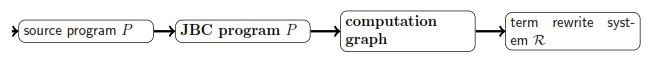
\includegraphics[angle=0,width=10cm]{big_picture.jpg}
                       \caption{Vision of the Big Picture.}
        \end{figure}
        \end{block}
	\begin{block}{My part:}
		\begin{itemize}
			\item small transformation tool for Jinja bytecode programs.
			\item input  = Jinja bytecode program
			\item output = finite computation graph
		\end{itemize}
	\end{block}
}

\frame{
        \frametitle{\textbf{Abstract States I}}
        \begin{block}{Why abstraction?}
                \begin{itemize}
                        \item all reachable states inside a program can not be computed because those are infinite.
                        \item using suitable abstractions, the computation graph becomes finite.
                \end{itemize}
        \end{block}
        \begin{block}{Difference between concrete and abstract states:}
                \begin{itemize}
                        \item abstract class variable, abstract integer value, abstract boolean value.
                        \item sharing information.
                        \item concrete state: no abstract variables, all addresses on the heap can't be shared further.
                \end{itemize}
        \end{block}
}

\frame{
        \frametitle{\textbf{Abstract States II}}
        \begin{block}{Instance concept:}
                \begin{itemize}
                        \item important when analysing loops.  
			\item when reaching a node again, check whether the new state is an instance of the state visited before. 
                \end{itemize}
        \end{block}
	\begin{block}{Example:}
	\begin{figure}[h!]
        \centering
        \begin{tikzpicture}[node distance=1.5cm,auto, scale=0.6, transform shape]
        \def\mshift{1.5cm}
        \def\mshiftx{1.15cm}
        \node (r0)                                  { reg0 };
        \node (r1)   at (r0)  [xshift=2cm]      { reg1 };
        \node (r2)   at (r1)  [xshift=2cm]      { reg2 };
        \node (rr0)  at (r2)  [xshift=5cm]          { reg0 };
        \node (rr1)  at (rr0) [xshift=2cm]      { reg1 };
        \node (rr2)  at (rr1) [xshift=2cm]      { reg2 };

        \node (a0)  [below of=r0]  { $a_0 \colon \m{List}$ };
        \node (a1)  [below of=r2]  { $a_1 \colon \m{List}$ };
        \node (a2)  [below of=r1]  { $a_2 \colon list$ };
        \node (a6)  [below of=rr2] { $a_6 \colon \m{List}$ };
        \node (a7)  [below of=rr1]  { $a_7 \colon list$ };
        \node (a8)  [below of=rr0] { $a_8 \colon \m{List}$ };

        \node (iival) [below of=a0, xshift = 1cm] { $AbsInt$ };
        \node (a4)    [below of=a1, xshift= -1cm] { $a_4 \colon list$ };
        \node (ival)  [below of=a1, xshift = 1cm] { $AbsInt$ };
        \node (a9)    [below of=a8, xshift= -1cm] { $a_9 \colon list$ };
        \node (a10)    [below of=a6, xshift= -1cm] { $a_{10} \colon list$ };
        \node (ival1)  [below of=a6, xshift = 1cm] { $AbsInt$ };
        \node (ival2)  [below of=a8, xshift = 1cm] { $AbsInt$ };

        \draw (r0) -- (a0);
        \draw (r1) -- (a2);
        \draw (r2) -- (a1);
        \draw (rr0) -- (a8);
        \draw (rr1) -- (a7);
        \draw (rr2) -- (a6);

        \draw (a0) edge [bend left =20]node [xshift=3ex] {\footnotesize next} (a1);
        \draw (a0) edge [bend left =45] node [xshift=1ex] {\footnotesize val} (iival);
        \draw (a1) edge [bend right =45]node [xshift=1ex] {\footnotesize next} (a4);
        \draw (a1) edge [bend left =45] node [xshift=1ex] {\footnotesize val} (ival);
        \draw (a8) edge [bend right =45] node [xshift=1ex] {\footnotesize next} (a9);
        \draw (a8) edge [bend left =45] node [xshift=1ex] {\footnotesize val} (ival2);
        \draw (a6) edge [bend right =45] node [xshift=1ex] {\footnotesize next} (a10);
        \draw (a6) edge [bend left =45] node [xshift=1ex] {\footnotesize val} (ival1);

        \end{tikzpicture}
        \caption{States \emph{s27} and \emph{s49} from List example.}
        \label{fig:morph-inststates}
        \end{figure}
	
	\end{block}
}


\frame{
	\frametitle{\textbf{Computation Graph I}}
	A state of the Jinja Virtual Machine is a pair consisting of heap and frame. 
	
	\begin{block}{Heap:}
		\begin{itemize}
			\item   global memory.
			\item 	mapping from addresses to objects.  
			\item 	object has a class name and a fieldtable(= mapping from (class name, fieldid) to a Jinja value) or is an abstract class variable. 
		\end{itemize}
	\end{block}
	\begin{block}{Frame:}
		\begin{itemize}
			\item represents execution environment of a method. 
			\item (opstack  , registers, class name, method name, pc)
		\end{itemize}
	\end{block}
}

\frame{
	\frametitle{\textbf{Computation Graph II}}
	\begin{block}{Brief description:}
		\begin{itemize}
			\item $G=(V,E)$. V are abstract states and E are the edges.
			\item abstract states: set of concrete states of the JVM. 
			\item edges: symbolic evaluation together with refinement and abstraction steps. 
			\item directed and acyclic graph.
			\item representation of all runs of a JBC program.
		\end{itemize}
	\end{block}
}

\frame{
	\frametitle{\textbf{Computation Graph III}}
	\begin{block}{Restrictions:}
	\begin{itemize}
		\item non-recursive methods. 
		\item tree-shaped objects.
	\end{itemize}
	\end{block}
	\begin{block}{Why computation graphs?}
	The motivation behind computation graphs is that they can handle all aspects of Jinja that cannot be expressed easily in \emph{term rewriting systems}.
	\end{block}
}

\frame{
	\frametitle{\textbf{Computation Graph IV}}
         \begin{figure}[H]\centering
                        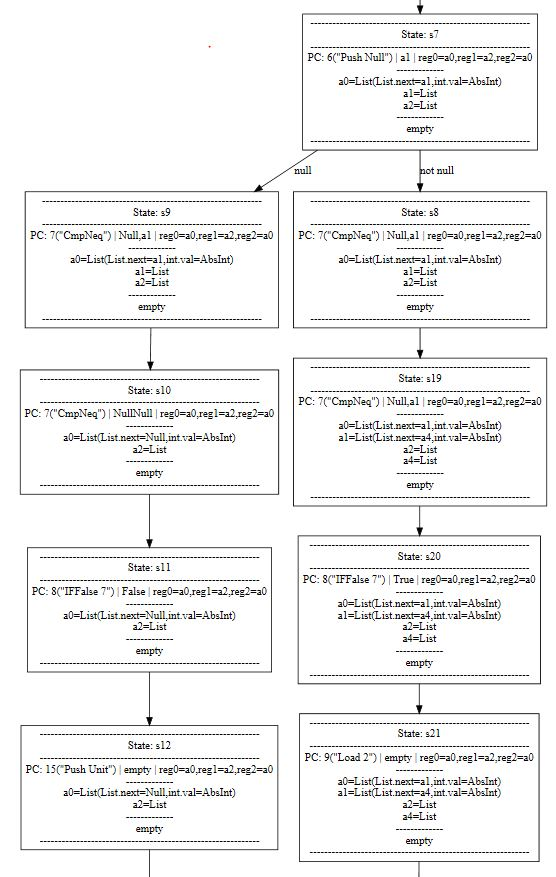
\includegraphics[scale=0.27]{compgraph-list.jpg}
                        \caption{Parts of the Computation Graph for the List example.}
         \end{figure}
}

\frame{
        \frametitle{\textbf{Transformation Tool I}}
        \begin{block}{Introduction:}
                \begin{itemize}
                        \item written in Haskell. 
			\item binary for Linux OS. 
                        \item converts JBC program into computation graph. 
                \end{itemize}
        \end{block}
	\begin{block}{Approach:}
                \begin{enumerate}
                        \item execute instruction from the instruction list until program reachs a loop. 
                        \item abstract states (summarizing) and perform loop again. 
			\item program termintes when the $PC$ reaches end of the instruction list or an instance has been found during analysis of a loop.                 \end{enumerate}
        \end{block}
}

\frame{
        \frametitle{\textbf{Transformation Tool II}}
        \begin{block}{Additional features:}
                \begin{itemize}
                        \item provides interface between the computation graph data type and GraphViz API. 
			\item cycle detection inside the heap. 
			\item integrated parser that transforms the JBC program into a well-defined data type used for internal representation by the computation graph.
                \end{itemize}
        \end{block}
}


\begin{frame}[fragile]
	\frametitle{\textbf{Example I}}
	\begin{block}{Source-code:}
		\begin{figure}[h!]
	        \centering
	        \begin{lstlisting}[numbers=none,basicstyle=\scriptsize\ttfamily]
		class List{
		List next;
		int val;
	
		unit append(List ys){
		        List cur = this;
		        while(cur.next!=null){
		                cur = cur.next;
		        };
	        cur.next = ys;
		}
		}
	        \end{lstlisting}
        	\caption{The Jinja source code for the method \emph{append} declared in the class \emph{List}.}
	        \label{fig:list-source}
	        \end{figure}
	\end{block}
\end{frame}

\begin{frame}[fragile]
        \frametitle{\textbf{Example II}}
        \begin{block}{Bytecode:}
                \begin{figure}[h!]
		\centering
                \begin{lstlisting}[numbers=none,basicstyle=\scriptsize\ttfamily]
		0:  Load 0               12: Push unit
		1:  Store 2              13: Pop
		2:  Push unit            14: Goto -10
		3:  Pop                  15: Push unit
		4:  Load 2               16: Pop
		5:  Getfield next List   17: Load 2
		6:  Push null            18: Load 1
		7:  CmpNeq               19: Putfield next List
		8:  IfFalse 7            20: Push unit
		9:  Load 2               21: Return
		10: Getfield next List
		11: Store 2
		\end{lstlisting}
	        \caption{The List JBC-program.}
	        \label{fig:list-jbc}
                \end{figure}
        \end{block}
\end{frame}

\begin{frame}
        \frametitle{\textbf{Example III}}
        \begin{block}{}
	\begin{center}
	Live presentation
	\end{center}
        \end{block}
\end{frame}

\frame{
	\frametitle{\textbf{Difficulties}}
	\begin{block}{}
	\begin{itemize}
		\item erros in theory led to problems in implemenation. 
		\item abstraction (implementation of summarizing).
		\item implementing unification between addresses on the heap.
		\item implementing morphism between states.
		\item termination of the program.  
	\end{itemize}
	\end{block}	

}

\frame{
	\frametitle{\textbf{Schedule}}
	\begin{tikzpicture}
	\usetikzlibrary[positioning];
	\tikzstyle{evnode}=[anchor=north west,draw=blue, shape=rectangle,rounded corners];
	\tikzstyle{tnode}=[draw, shape=circle, fill, color=blue];
	\tikzstyle{dnode}=[anchor=west,font=\small\color{blue}];

	\node[tnode] (nt0) at (0,0) {};
	\node[tnode] (nt1) at (0,-4.0) {};
	\node[tnode] (nt2) at (0,-6) {};

	\node[dnode] (ini) at (0.5,0) {13\textsuperscript{th} March 2012: Initial presentation};
	\node[dnode] (sem) at (0.5,-4.0) {3\textsuperscript{th} September 2012: End of programing};
	\node[dnode] (fin) at (0.5,-6) {16\textsuperscript{th} October 2012: Final presenation};

	\node[evnode] (ev1) at (0.7,-0.3) {
	\begin{minipage}{6cm}
	  \begin{itemize}
		\item March: Reading papers
		\item April: JBC instruction set, refinements
		\item May - June: Morphism, unification and instance 
		\item July - August: Summarizing
	  \end{itemize}
	\end{minipage}
	};
			
	\node[evnode] (ev2) at (0.7,-4.3) {
	\begin{minipage}{6cm}
	  \begin{itemize}
	    \item September: Writing thesis, testing, final presentation 
	  \end{itemize}
	\end{minipage}
	};

	\draw[->] (nt0) -- (nt1);
	\draw[->] (nt1) -- (nt2);
	
	\end{tikzpicture}

}



\frame{
	\frametitle{\textbf{Conclusion}}
	\begin{block}{Achievements:}
		\begin{itemize}
			\item transformation of JBC program into finite computation graph.
			\item implementation of the theoritical approach from \cite{paper-uibk}.
			\item generate finite output with the help of abstraction (summarizing).   
		\end{itemize}
	\end{block}	
	\begin{block}{Future work:}
		\begin{itemize}
			\item improve performance of the tool. 
			\item output of Dot file representation.
			\item use of recursive methods in the program.
			\item implementation of transformation step from computation graph to $TRS$. 
		\end{itemize}
	\end{block}	
	
}

\frame{
	\frametitle{\textbf{Bibliography}}
	\bibliography{biblio}
	\bibliographystyle{plain}
}

\frame{
	\frametitle{\textbf{End}}
	\begin{center}
	Thank you for your attention! \\
	Questions?
	\end{center}

	
}


\end{document}
